\documentclass[11pt]{article}
\usepackage[utf8]{inputenc}
\usepackage{lmodern}
\usepackage[a4paper,margin=0.95in]{geometry}
\usepackage{amsmath,amssymb,bm}
\usepackage{graphicx}
\usepackage{booktabs}
\usepackage{array}
\usepackage{microtype}
\usepackage{hyperref}
\usepackage{titlesec}
\titlespacing*{\section}{0pt}{1.0ex}{0.5ex}
\titlespacing*{\subsection}{0pt}{0.7ex}{0.3ex}
\setlength{\parskip}{2pt}
\setlength{\parindent}{0pt}

\title{\textbf{Multi-Head LUT --- optimisation techniques\\
\large math reference and apples-to-apples experiments}}
\author{}
\date{\today}

\begin{document}
\maketitle

\section*{Scope}

This short note first lays out the formal description of two Multi-Head
LUT families (\S\,\ref{sec:math}), then reports a set of like-for-like
training runs (\S\,\ref{sec:exp}) that probe the specific design choices
isolated in that description. All experiments fix every architectural and
optimisation hyperparameter except the LUT forward/backward recipe;
the only variable across each comparison group is the choice of smooth
surrogate from the math section.

% ==========================================================================
\section{Math --- the two Multi-Head LUT families}\label{sec:math}

Two families of LUT modules sit on top of the same discrete idea: replace a
learned linear projection with a learned row-lookup, indexed by signs of
pairwise input comparisons. The two families differ in \textbf{how they
smooth the discrete forward for training} --- the \S\,\ref{sec:can} family
uses an \emph{uncertainty kernel} (the original manifesto formulation),
the \S\,\ref{sec:soft} family uses a \emph{softmax over all rows of the
table} (the newer construction).

\subsection{Basics}\label{sec:basics}

A Multi-Head LUT replaces a linear projection $y=Wx$ with a learned
table-lookup. Input $x\in\mathbb{R}^{d_{\mathrm{in}}}$, output
$y\in\mathbb{R}^{H\times n_{\mathrm{out}}}$.

A module has $H$ heads (\texttt{n\_heads}) and \texttt{tph} tables per head.
Total tables $T=H\cdot\mathrm{tph}$. Each table $t$ owns a weight tensor
\[
  W_t\in\mathbb{R}^{K\times n_{\mathrm{out}}},\qquad K=2^{\mathrm{NAP}},
\]
where NAP (number of anchor pairs) is the per-table input bit-width.

\paragraph{Anchor pairs.} For each table, two integer lists are sampled once
at init:
\[
  a_t,\,b_t\in[0,d_{\mathrm{in}})^{\mathrm{NAP}}
\]
with \emph{balanced full coverage} (each input dimension participates in
equally many pairs across the module). Anchors are buffers; they do not
move during training.

\paragraph{Per-table row index} (the discrete part, used in every variant
below):
\[
  d_t[i] = x[a_t[i]] - x[b_t[i]],\quad
  \mathrm{bits}_t[i] = \mathbf{1}[d_t[i]>0],\quad
  \mathrm{chosen}_t = \sum_{i=0}^{\mathrm{NAP}-1}\mathrm{bits}_t[i]\,2^{\mathrm{NAP}-1-i}\in[0,K).
\]

\paragraph{Module output} per head sums table contributions:
\[
  y[h,:] = \sum_{t\in\text{head }h} \text{out}_t.
\]

The $\text{out}_t\in\mathbb{R}^{n_{\mathrm{out}}}$ formula differs across
\S\,\ref{sec:can} and \S\,\ref{sec:soft}. Defaults: $\mathrm{NAP}{=}6$,
$K{=}64$.

\paragraph{Aside: the straight-through estimator (STE).}
The discrete map $x\mapsto\mathrm{chosen}_t$ is not differentiable --- it is
constant in $x$ between sign flips and jumps at the flips, so its true
gradient is zero almost everywhere. To still train the module by
gradient descent one substitutes a \emph{surrogate} gradient: the
forward returns the hard value, but the backward pass acts as if some
smooth function had been computed. The standard implementation is
the \emph{straight-through estimator}: write the output as
\[
  \text{out} \;=\; \text{out}_{\mathrm{hard}}
                 \;+\; \bigl(\text{out}_{\mathrm{soft}}
                            - \text{out}_{\mathrm{soft}}.\mathrm{detach}()\bigr),
\]
where $\text{out}_{\mathrm{soft}}$ is some \emph{differentiable} surrogate
of $\text{out}_{\mathrm{hard}}$ and $.\mathrm{detach}()$ marks a copy on
which autograd will not back-propagate. Numerically the bracketed term is
$0$, so the forward equals $\text{out}_{\mathrm{hard}}$. But during the
backward pass autograd sees $\partial \text{out}/\partial x =
\partial \text{out}_{\mathrm{soft}}/\partial x$, so the gradient flows
through the soft surrogate. The choice of $\text{out}_{\mathrm{soft}}$ is
the whole story --- \S\,\ref{sec:can} and \S\,\ref{sec:soft} are two
different choices for it on top of the same hard $\mathrm{chosen}_t$.

% --------------------------------------------------------------------------
\subsection{Canonical \texttt{MultiHeadLUT} --- the manifesto formulation}
\label{sec:can}

The forward is a row gather; the soft variant blends the chosen row with the
$K'$ nearest rows, weighted by an \emph{uncertainty kernel}. The hard
variant is the manifesto's deployed forward.

\subsubsection{Forward --- hard (the manifesto)}\label{sec:can-hard}
\[
  \text{out}_t = W_t[\mathrm{chosen}_t,\,:]
\]
NAP comparisons, one row gather, no multiplications. Exactly the manifesto's
deployed module.

\subsubsection{Forward --- soft (uncertainty blend)}\label{sec:can-soft}

The $K'$ nearest rows are obtained by 1-bit-flipping the $K'$ anchor
positions with the smallest $|d_t[i]|$. Call them $\mathrm{pos}_1,\ldots,\mathrm{pos}_{K'}$
(sorted by $|d_t[\mathrm{pos}_i]|$ ascending) and define
\[
  \mathrm{alt}_{t,i} = \mathrm{chosen}_t\oplus 2^{\mathrm{NAP}-1-\mathrm{pos}_i},
  \qquad
  d_{t,i}^{\mathrm{alt}} = d_t[\mathrm{pos}_i].
\]
The \emph{uncertainty kernel} (inverse-$L^1$, manifesto default):
\[
  u(|d|) = \frac{\beta}{1+|d|},\quad \beta=0.5\ \text{(\texttt{uncertainty\_bias})}.
\]
Per-row blending weights:
\[
  \alpha_{t,i}^{\mathrm{alt}} = \frac{u(|d_{t,i}^{\mathrm{alt}}|)}{K'},\qquad
  \alpha_t^{\mathrm{main}} = 1-\sum_{i=1}^{K'}\alpha_{t,i}^{\mathrm{alt}}.
\]
Forward soft:
\[
  \text{out}_t \;=\; \alpha_t^{\mathrm{main}}\,W_t[\mathrm{chosen}_t,:]
                 \;+\; \sum_{i=1}^{K'}\alpha_{t,i}^{\mathrm{alt}}\,W_t[\mathrm{alt}_{t,i},:].
\]

\paragraph{Tradeoff vs.\ hard.} Forward now reads $1{+}K'$ rows per table
and computes a $(K'{+}1)$-term linear combination ---
$O(K'\cdot n_{\mathrm{out}})$ multiplications per table per token. The
manifesto's ``no multiplications at inference'' property is lost in soft
mode; it is a training-only forward unless one accepts the
bandwidth/compute cost at deploy. The case $K'{=}1$ is the manifesto's
soft formulation; $K'{=}3$ is the default in our experiments.

\subsubsection{Backward}\label{sec:can-bwd}

Forward soft is differentiable through $u$ (since $\alpha^{\mathrm{main}},\alpha^{\mathrm{alt}}_i$
depend on $|d_{t,i}^{\mathrm{alt}}|$) and the weights enter linearly --- plain
autograd.

Uncertainty derivative:
\[
  \frac{\partial u}{\partial |d|} = -\frac{\beta}{(1+|d|)^2},\quad
  \frac{\partial |d|}{\partial d} = \mathrm{sign}(d),\quad
  \frac{\partial u}{\partial d} = -\frac{\beta\,\mathrm{sign}(d)}{(1+|d|)^2}.
\]
Define $g_t^{\mathrm{main}}=\langle g^{\mathrm{out}}_t,\,W_t[\mathrm{chosen}_t,:]\rangle$ and
$g_{t,i}^{\mathrm{alt}}=\langle g^{\mathrm{out}}_t,\,W_t[\mathrm{alt}_{t,i},:]\rangle$.
Since $\partial\alpha^{\mathrm{main}}/\partial\alpha^{\mathrm{alt}}_i=-1$ and
$\alpha^{\mathrm{alt}}_i=u(|d_{t,i}^{\mathrm{alt}}|)/K'$, the chain gives
\[
  \frac{\partial L}{\partial d_{t,i}^{\mathrm{alt}}}
  = (g_{t,i}^{\mathrm{alt}}-g_t^{\mathrm{main}})\cdot
    \Bigl(-\frac{\beta\,\mathrm{sign}(d_{t,i}^{\mathrm{alt}})}{(1+|d_{t,i}^{\mathrm{alt}}|)^2}\Bigr)\cdot\frac{1}{K'}.
\]
Scatter to anchors: $\partial L/\partial x[a_t[\mathrm{pos}_i]]\mathrel{+}=
\partial L/\partial d_{t,i}^{\mathrm{alt}}$, with $-$ for the $b$-leg.

Weight gradient (linear in $\alpha$'s):
\[
  \frac{\partial L}{\partial W_t[\mathrm{chosen}_t,:]}\mathrel{+}=\alpha_t^{\mathrm{main}}\,g^{\mathrm{out}}_t,
  \qquad
  \frac{\partial L}{\partial W_t[\mathrm{alt}_{t,i},:]}\mathrel{+}=\alpha_{t,i}^{\mathrm{alt}}\,g^{\mathrm{out}}_t.
\]

\paragraph{Note on \texttt{smooth\_mode}.} The $x$-gradient chain above is
\emph{independent} of \texttt{smooth\_mode}. The forward toggle (hard pick
vs.\ soft blend) only changes which combination of rows is \emph{output};
the backward still routes the same uncertainty-kernel gradient to $x$.
What \texttt{smooth\_mode} changes in the backward is the
\textbf{weight-gradient distribution}: when \texttt{True}, weight grad is
spread across chosen + $K'$ alts with the $\alpha$'s; when \texttt{False},
weight grad is a hard \texttt{index\_add} at the chosen row only. In the
hard-mode implementation a standard STE wrapper is used:
$\text{out} = \text{main} + (\text{soft} - \text{soft.detach()})$, so the
forward value equals $W[\mathrm{chosen}]$ but the soft chain still flows to
$x$.

% --------------------------------------------------------------------------
\subsection{\texttt{SoftMultiHeadLUT} --- softmax over all rows}\label{sec:soft}

A different soft mechanism. Instead of blending chosen with $K'$ nearby
rows by uncertainty, \emph{score every row of the table against $x$ via a
softmax}, then either pick the top row (hard, STE) or take the soft
mixture (soft).

\subsubsection{Soft signs $\times$ bit matrix $\to$ softmax}\label{sec:soft-construct}

Replace each binary bit by a smooth proxy:
\[
  p_t[i] = \frac{d_t[i]}{T_{\mathrm{soft}} + |d_t[i]|}\in(-1,+1).
\]
$T_{\mathrm{soft}}>0$ is a temperature: small $T_{\mathrm{soft}}$ makes $p$ nearly $\pm 1$;
large $T_{\mathrm{soft}}$ makes it nearly linear in $d$.

Define the \textbf{bit matrix} $B\in\{-1,+1\}^{\mathrm{NAP}\times K}$ ---
column $k$ is the $\pm 1$ expansion of integer $k$, MSB first:
$B[i,k]=+1$ if bit $(\mathrm{NAP}{-}1{-}i)$ of $k$ is $1$, else $-1$.

Row match scores (popcount-like at the hard limit):
\[
  \mathrm{ts}_t[k] = \sum_i p_t[i]\,B[i,k]\in[-\mathrm{NAP},+\mathrm{NAP}].
\]
Intuition: $\mathrm{ts}_t[k]$ is maximised at the integer $k$ whose bit pattern
agrees with $\mathrm{sign}(p_t)$. At the hard limit ($p\in\{\pm 1\}^{\mathrm{NAP}}$),
$\arg\max_k\mathrm{ts}_t[k] = \mathrm{chosen}_t$ of \S\,\ref{sec:basics} --- provably equal
at fp32. So this construction is a smooth interpolation between ``no
information'' (all $p{=}0\to$ uniform softmax) and ``the manifesto hard
pick'' (all $p{=}\pm 1\to$ ts maximised exactly at $\mathrm{chosen}_t$).

Soft selector:
\[
  \mathrm{sel}_t[k] = \mathrm{softmax}_k\bigl(\mathrm{ts}_t[:]/T_{\mathrm{sel}}\bigr)\in\Delta^{K-1}.
\]
$T_{\mathrm{sel}}>0$ is the row-selection temperature. Both temperatures are
log-parametrised ($T=\exp(\log T)$) and learnable.

\subsubsection{Forward --- hard (STE)}\label{sec:soft-hard}
\[
  \mathrm{chosen}_t = \arg\max_k \mathrm{ts}_t[k]\quad(\text{same integer as
\S\,\ref{sec:basics}}),\qquad
  \text{out}_t = W_t[\mathrm{chosen}_t,:].
\]
Numerically identical to \S\,\ref{sec:can-hard}. The standard STE in PyTorch:
$\mathrm{sel}_{\mathrm{through}} = \mathrm{sel}_{\mathrm{hard}} - \mathrm{sel}_t.\mathrm{detach}() + \mathrm{sel}_t$
(numerically $=\mathrm{sel}_{\mathrm{hard}}$); autograd flows through $\mathrm{sel}_t$.

\subsubsection{Forward --- soft (true mixture)}\label{sec:soft-soft}
\[
  \text{out}_t = \sum_k \mathrm{sel}_t[k]\,W_t[k,:].
\]
A full convex combination over all $K=2^{\mathrm{NAP}}$ rows. Output varies
smoothly with $x$ (no row jumps at sign flips). Cost: $K$ row reads, softmax
over $K$, $K$-term weighted sum --- only practical with small NAPs.

\subsubsection{Backward --- full soft (over all $K$ rows)}\label{sec:soft-bwd}

Plain autograd for \S\,\ref{sec:soft-soft}; STE wrapper for \S\,\ref{sec:soft-hard}
routes through the same chain. Closed form:
\[
\begin{aligned}
  g_t^{\mathrm{sel}}[k] &= \langle g^{\mathrm{out}}_t,\,W_t[k,:]\rangle,\\
  g_t^{z}[k] &= \frac{\mathrm{sel}_t[k]}{T_{\mathrm{sel}}}\Bigl(g_t^{\mathrm{sel}}[k] - \sum_j \mathrm{sel}_t[j]\,g_t^{\mathrm{sel}}[j]\Bigr),\\
  g_t^{p}[i] &= \sum_k g_t^{z}[k]\,B[i,k],\\
  g_t^{d}[i] &= g_t^{p}[i]\cdot \frac{T_{\mathrm{soft}}}{(T_{\mathrm{soft}}+|d_t[i]|)^2},\\
  \partial L/\partial x[a_t[i]] &\mathrel{+}= g_t^{d}[i],\qquad
  \partial L/\partial x[b_t[i]] \mathrel{-}= g_t^{d}[i].
\end{aligned}
\]
Weight gradient:
\[
  \text{\S\,\ref{sec:soft-hard} (STE):}\ \frac{\partial L}{\partial W_t[\mathrm{chosen}_t,:]}\mathrel{+}=g^{\mathrm{out}}_t;\qquad
  \text{\S\,\ref{sec:soft-soft} (soft):}\ \frac{\partial L}{\partial W_t[k,:]}\mathrel{+}=\mathrm{sel}_t[k]\,g^{\mathrm{out}}_t\ \text{for all }k.
\]
Temperature gradients (from the same chain):
\[
  \frac{\partial L}{\partial \log T_{\mathrm{sel}}} = -\sum_{t,k} g_t^{z}[k]\,\mathrm{ts}_t[k],\qquad
  \frac{\partial L}{\partial \log T_{\mathrm{soft}}} = -\sum_{t,i} g_t^{d}[i]\,d_t[i].
\]
Every row of every table contributes; saved-for-backward memory is
$O(B\cdot T\cdot K)$ for $\mathrm{sel}$ plus the $\mathrm{ts},p,d$ intermediates.

\subsubsection{Backward --- top-$K'$ approximation}\label{sec:soft-topk}

Compute $\mathrm{ts}_t$ then \textbf{mask} to $-\infty$ at every row outside
\[
  S_t = \{\mathrm{chosen}_t\}\cup \bigl\{\mathrm{chosen}_t\oplus 2^{\mathrm{NAP}-1-\mathrm{pos}_i}:i=1\ldots K'\bigr\},
\]
where $\mathrm{pos}_1,\ldots,\mathrm{pos}_{K'}$ are the $K'$ lowest-$|d|$ anchor positions
(same selection rule as \S\,\ref{sec:can-soft}). The softmax now
renormalises over only $1{+}K'$ rows; everything else in \S\,\ref{sec:soft-bwd}
is unchanged. Limits: $K'{=}0$ $\to$ $\mathrm{sel}=\delta_{\mathrm{chosen}}$
(weight grad is hard \texttt{index\_add}, but $x$-grad still flows through
the soft-sign Jacobian); $K'{=}\mathrm{NAP}$ $\to$ Hamming-1 ball
($\mathrm{NAP}{+}1$ rows total); $K'{=}K{-}1$ $\to$ recovers \S\,\ref{sec:soft-bwd}
exactly. The motivation is memory: \S\,\ref{sec:soft-bwd}'s $O(K)$ memory
becomes a bottleneck at large NAP or large batch; top-$K'$ keeps the same
softmax-chain math at $O(K')$ rows.

% --------------------------------------------------------------------------
\subsection{How \S\,\ref{sec:can} and \S\,\ref{sec:soft} relate}

Same discrete forward (hard pick at $\mathrm{chosen}_t$). Different smooth
surrogates.

\begin{center}\small
\begin{tabular}{>{\raggedright\arraybackslash}p{0.22\linewidth} >{\raggedright\arraybackslash}p{0.36\linewidth} >{\raggedright\arraybackslash}p{0.34\linewidth}}
\toprule
 & \S\,\ref{sec:can} uncertainty blend (manifesto) & \S\,\ref{sec:soft} softmax over rows \\
\midrule
Forward soft output & linear combination of chosen + $K'$ nearest rows, weighted by $1/(1+|d^{\mathrm{alt}}|)$ & softmax-weighted combination over all $K$ rows of $\mathrm{ts}=\text{soft-signs}\cdot B$ \\
$K'{=}1$ (or analog) & manifesto soft: blend chosen with one alt & no ``alts'' parameter; analog is \S\,\ref{sec:soft-topk} at $K'{=}1$ \\
Hard forward (\texttt{smooth=False} / \texttt{hard=True}) & out${=}W[\mathrm{chosen}]$; $\partial L/\partial x$ flows via uncertainty STE; weight grad is hard \texttt{index\_add} & out${=}W[\mathrm{chosen}]$ via $\mathrm{sel}_{\mathrm{hard}}-\mathrm{sel}_{\mathrm{soft}}.\mathrm{detach}()+\mathrm{sel}_{\mathrm{soft}}$ STE; $\partial L/\partial x$ flows via soft-sign chain; weight grad is hard \texttt{index\_add} \\
$x$-gradient source (soft mode) & flip-induced ``swap'' $g^{\mathrm{alt}}_i - g^{\mathrm{main}}$ scaled by $-\beta\mathrm{sign}(d^{\mathrm{alt}})/(1+|d^{\mathrm{alt}}|)^2$ & full softmax chain: every anchor position contributes $g^{d}_i\cdot T_{\mathrm{soft}}/(T_{\mathrm{soft}}+|d|)^2$ \\
Weight gradient (soft mode) & $\alpha^{\mathrm{main}}\,g^{\mathrm{out}}$ to chosen, $\alpha^{\mathrm{alt}}_i g^{\mathrm{out}}$ to each alt & $\mathrm{sel}_t[k]\,g^{\mathrm{out}}$ to \emph{every} row \\
Inference forward & \S\,\ref{sec:can-hard} (hard pick), no multiplications & \S\,\ref{sec:soft-hard} (hard pick, same as \S\,\ref{sec:can-hard}), no multiplications \\
Inference compute (soft mode, if used) & $(1{+}K')\cdot n_{\mathrm{out}}$ mults per table & $K\cdot n_{\mathrm{out}}$ mults per table (impractical) \\
\bottomrule
\end{tabular}
\end{center}

Both families collapse to the same hard inference (one row gather per
table). They are alternative training-time smoothings of that hard forward.

\clearpage
% ==========================================================================
\section{Experimental comparison}\label{sec:exp}

We compare two groups of runs. The first isolates the \emph{backward} choice
of the smooth surrogate (\S\,\ref{sec:math}: \S1 vs.\ \S2 vs.\ \S2.5) at a
small, well-behaved 43M LUT-LM. The second isolates the \emph{forward} choice
(\S\,\ref{sec:math}: \S2.2 hard STE pick vs.\ \S2.3 true soft mixture) at our
best-performing 89M LUT-LM architecture.

All training hyperparameters --- optimiser, learning rates, weight decay,
warmup, total tokens, batch size, NAP and tables-per-head, anchor seed ---
are identical inside each group. Only the LUT module class / forward
mode / backward mode differs. Both groups use the same vocabulary and
validation set.

% --------------------------------------------------------------------------
\subsection{Group A --- backward mechanism (43M, bs=16)}
\label{sec:expA}

\textbf{Architecture.} Pre-LUT residual stream $D{=}384$, embedding stream
$E{=}48$, $L{=}6$ layers, $H{=}6$ heads, $d_{qk}{=}64$, $d_v{=}8$, RoPE on
$(q,k)$. The four LUT modules per layer (\texttt{qkv\_lut}, \texttt{v\_lut},
\texttt{out\_proj}, \texttt{residual\_lut}) use NAP$/$tph
$=6/16$, $8/32$, $8/128$, $6/64$ respectively. 43M parameters,
\texttt{argmax\_noise\_eps}${=}0$, $\text{bs}{=}16$, 8K steps.

\textbf{Knob.} Each LUT module is one of:

\begin{itemize}\itemsep0pt
\item \textbf{exp365} --- \texttt{TinyMHLut}, \texttt{backward\_mode='soft'}.
    Hard STE forward (\S\,\ref{sec:soft-hard}), full
    softmax-over-rows backward (\S\,\ref{sec:soft-bwd}).
    \emph{This is the \S2 mechanism at full $K=2^{\mathrm{NAP}}$.}
\item \textbf{exp403} --- \texttt{TinyMHLut}, \texttt{backward\_mode='soft\_topk'},
    $K'=\text{NAP}$. Top-$K'$ approximation of \S\,\ref{sec:soft-topk}; the
    softmax is masked to the chosen row plus the full 1-bit-flip Hamming-1
    ball ($\mathrm{NAP}{+}1$ rows).
\item \textbf{exp402} --- \texttt{TinyMHLut}, \texttt{backward\_mode='soft\_topk'},
    $K'=3$. Same as exp403 but only the 3 lowest-$|d|$ neighbours.
\item \textbf{exp386} --- legacy \texttt{MultiHeadLut},
    \texttt{n\_alternatives=3}, \texttt{smooth\_mode=True}.
    \emph{This is the \S1 mechanism}: soft forward is a
    $(1{+}K')$-row uncertainty blend, backward is the closed-form
    kernel chain of \S\,\ref{sec:can-bwd}.
\item \textbf{exp351} --- \texttt{TinyMHLut}, \texttt{backward\_mode='ste'},
    $n_{\mathrm{alt}}{=}3$. \S1.1 hard pick forward + \S1.3 uncertainty-kernel
    STE backward.
    \emph{Caveat:} this run also turned on small bernoulli flip-noise
    (\texttt{argmax\_noise\_eps}${=}0.002$) and was killed at step 4K because
    the trajectory was clearly behind every other recipe. Shown for context
    only.
\end{itemize}

\begin{figure}[h]
\centering
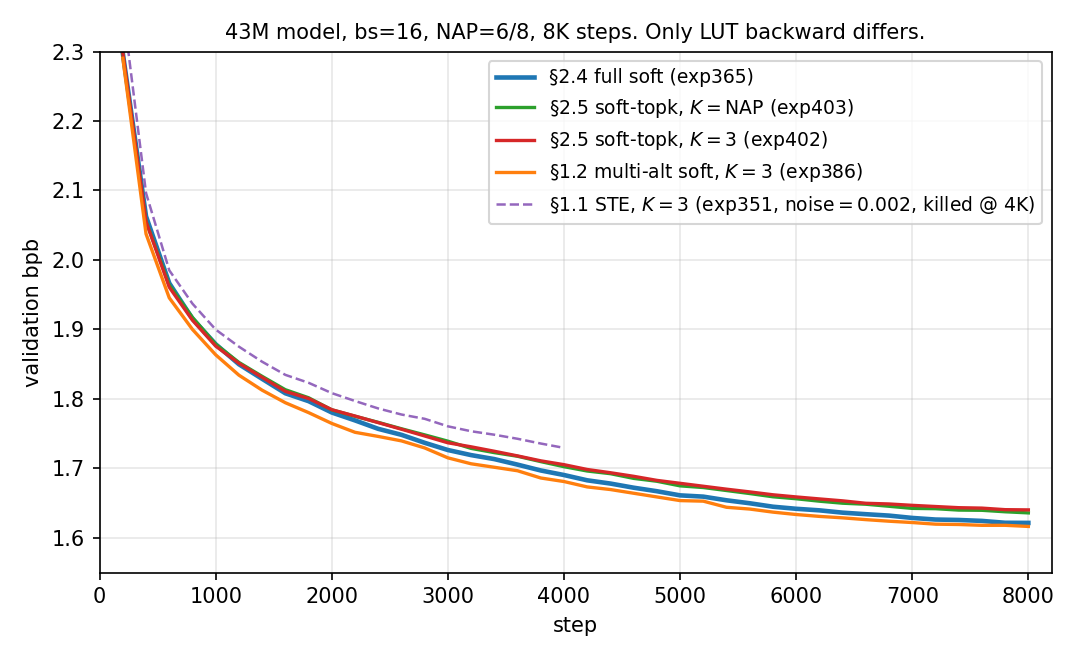
\includegraphics[width=0.92\linewidth]{figs/optech_43m_curves.png}
\caption{43M LUT-LM, all hyperparameters fixed except the LUT optimisation
recipe (mapped to the math section). Final bpb in Table~\ref{tab:A}.}
\label{fig:A}
\end{figure}

\begin{table}[h]
\centering
\small
\begin{tabular}{l l l c c}
\toprule
exp & math ref.\ & recipe & rows used / table & final val bpb \\
\midrule
exp365 & \S\,\ref{sec:soft-bwd}     & soft (full)              & $K{=}2^{\mathrm{NAP}}$ ($64$ or $256$) & $1.6215$ \\
exp403 & \S\,\ref{sec:soft-topk}    & soft-topk $K'{=}\mathrm{NAP}$ & $\mathrm{NAP}{+}1$ (7 or 9) & $1.6359$ \\
exp402 & \S\,\ref{sec:soft-topk}    & soft-topk $K'{=}3$       & $4$ & $1.6402$ \\
\midrule
exp386 & \S\,\ref{sec:can-bwd}      & multi-alt soft, $K'{=}3$ & $4$ (soft blend) & $\mathbf{1.6164}$ \\
exp351 & \S\,\ref{sec:can-bwd}      & multi-alt STE, $K'{=}3$  & $1$ fwd, $3$ alts bwd & $1.7295$ (4K, killed) \\
\bottomrule
\end{tabular}
\caption{Group A. Bold marks the lowest final bpb.}
\label{tab:A}
\end{table}

\textbf{Reading.}
(i) The \emph{soft-topk} approximation of \S\,\ref{sec:soft-topk} consistently
underperforms the full \S\,\ref{sec:soft-bwd} softmax-over-rows, but the gap
is small ($\sim$0.015 bpb) and shrinks as $K'\!\uparrow$; the Hamming-1 ball
($K'{=}\mathrm{NAP}$) recovers most of the loss for $\sim$10\% of the FLOPs.
(ii) The legacy \S1 uncertainty-blend (exp386, $K'{=}3$) is the strongest
recipe in this group --- about $0.005$ bpb \emph{better} than the full
\S2 softmax, at $\sim K/K'{\sim}16\times$ less backward compute. This is the
first evidence at LUT-LM scale that the \S1 forward smoothing and
\S2 backward are not interchangeable: the localised
$1/(1{+}|d|)$ kernel survives, and at this scale, beats the global softmax.
The win is not free at \emph{inference}, however: exp386's forward reads
$1{+}K'{=}4$ rows per table (vs.\ 1 for every other recipe in the group)
and performs $(K'{+}1)\cdot n_{\mathrm{out}}$ multiplications per table per
token. The manifesto's ``no multiplications, one row gather'' inference
property is forfeited --- so exp386 trades $\sim 4\times$ inference
bandwidth and a dense MAC pass for its 0.005 bpb. The other four recipes
all use the hard pick at deploy and keep the bandwidth-1, multiplication-0
inference forward intact (the \S2 cousins via \S\,\ref{sec:soft-hard}'s
STE, the \S1 hard STE via \S\,\ref{sec:can-hard}).
(iii) Going all the way to the hard STE (\S1.1 + \S1.3 with no soft forward)
diverges; even with noise injection on top, exp351 is $\gtrsim$0.1 bpb behind
at the same step count.

% --------------------------------------------------------------------------
\subsection{Group B --- forward mechanism at SOTA scale (89M, bs=16)}
\label{sec:expB}

\textbf{Architecture.} Our best-performing LUT-LM: dual-stream
($E{=}64$ ranking carrier + $D{=}384$ residual), fused
\texttt{qkv\_lut} (NAP$/$tph${=}6/64$) with a shallow $V$-branch,
separate \texttt{v\_lut} ($6/256$), \texttt{out\_proj} ($6/1024$),
and a pre-residual \texttt{residual\_lut} ($6/128$). 89.4M parameters,
$\text{bs}{=}16$, 8K steps, identical optimiser hyperparameters.

\textbf{Knob.} The four LUT modules per layer use either:

\begin{itemize}\itemsep0pt
\item \textbf{exp428} --- \texttt{TinyMHLut}, \texttt{backward\_mode='soft'}.
  \emph{Forward}: hard STE pick (\S\,\ref{sec:soft-hard}), output $= W[\text{chosen}, :]$.
  \emph{Backward}: full softmax-over-rows (\S\,\ref{sec:soft-bwd}).
\item \textbf{exp444} --- \texttt{SoftMultiHeadLUT}, \texttt{hard=False}.
  \emph{Forward}: true soft mixture (\S\,\ref{sec:soft-soft}),
  output $= \sum_k \mathrm{sel}_t[k] \cdot W[k,:]$.
  \emph{Backward}: identical softmax-chain to exp428 (just plain autograd
  through the same chain).
\end{itemize}

The two runs share their backward math; they differ only in whether the
forward observed by the rest of the model is a hard row or a convex
combination over all $2^{\mathrm{NAP}}$ rows.

\begin{figure}[h]
\centering
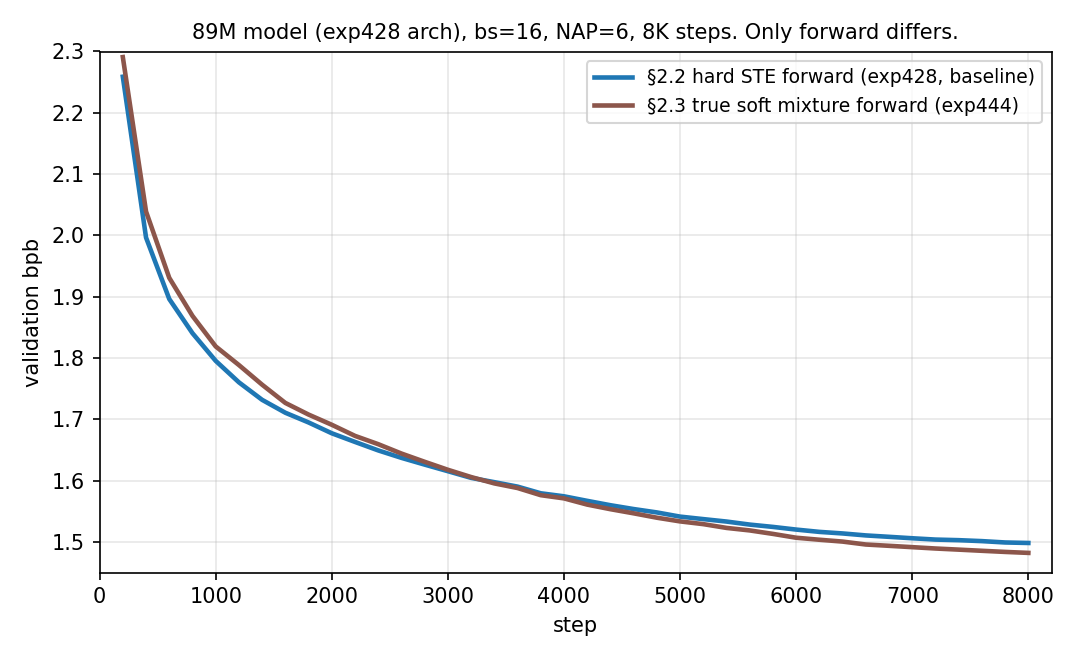
\includegraphics[width=0.92\linewidth]{figs/optech_89m_curves.png}
\caption{89M LUT-LM (exp428 architecture). The only change is the LUT
\emph{forward}: hard STE pick (exp428, blue) vs.\ true soft mixture
over all $K=64$ rows (exp444, brown).}
\label{fig:B}
\end{figure}

\begin{table}[h]
\centering
\small
\begin{tabular}{l l c c c}
\toprule
exp & forward type & rows/token & wall time (h, single A100) & final val bpb \\
\midrule
exp428 & hard STE pick (\S\,\ref{sec:soft-hard}) & $1$ & $0.41$ & $1.4983$ \\
exp444 & soft mixture (\S\,\ref{sec:soft-soft}) & $K{=}64$ & $2.12$ & $\mathbf{1.4821}$ \\
\bottomrule
\end{tabular}
\caption{Group B. Same backward chain, only the forward differs.}
\label{tab:B}
\end{table}

\textbf{Reading.} The interesting feature of Figure~\ref{fig:B} is the
\emph{crossover}: exp444 starts about $0.03$ bpb \emph{behind} exp428
(step 200: $2.29$ vs.\ $2.26$), the gap narrows monotonically, the two
curves cross around step $3{,}300$ ($1.61$ vs.\ $1.61$), and exp444
then pulls ahead, finishing $0.016$ bpb in front at step $8{,}000$
($1.482$ vs.\ $1.498$). The gap is still widening at the end of training
(growing from $-0.0154$ at step $7{,}800$ to $-0.0162$ at step $8{,}000$),
so the soft-mixture trajectory has not saturated. The crossover is not
dramatic, but it is consistent: with identical backward chain and
optimiser, the soft \S\,\ref{sec:soft-soft} forward pays an early
training-loss tax for routing the downstream stack through a smooth
convex combination, then converts that into a faster late slope. The
suggestion --- modest at this run length, but the direction is clear ---
is that the soft-forward architecture has more long-run headroom than
the hard STE pick at this scale.

% --------------------------------------------------------------------------
\subsection{Takeaways}

\begin{enumerate}\itemsep0pt
\item exp386 (\S1 uncertainty-blend forward, $K'{=}3$) and exp365 (\S2
  hard-pick forward, full softmax backward) end up on essentially the
  \emph{same trajectory}: exp386 wins by only $0.005$ bpb at step 8K and
  the two validation curves sit on top of each other for most of training.
  That marginal win is paid for very dearly --- exp386's forward reads
  $1{+}K'{=}4$ rows per table and performs a dense MAC pass at every
  layer, both at training \emph{and} at inference. exp365 keeps the
  manifesto's $\text{bandwidth}{=}1$, $\text{mult}{=}0$ inference forward
  intact. Read pragmatically, this says the \S1 soft-forward smoothing
  is \emph{not} worth its inference cost over the \S2 hard-pick +
  soft-backward recipe at this scale; the two smoothings produce the
  same minimum, so prefer the one whose deploy forward is cheap.
\item Top-$K'$ approximations of the \S2 chain (\S2.5) are cheap but lossy.
  Most of the gap is recovered by the Hamming-1 ball.
\item At our SOTA architecture the \S2 \emph{forward} matters as well as
  the backward, and exp428 vs.\ exp444 shows a clear (if not dramatic)
  \emph{crossover}: the soft mixture starts $\sim$0.03 bpb behind, the
  curves cross near step 3{,}300, and the soft mixture finishes
  $0.016$ bpb ahead with the gap still widening. The soft-forward
  architecture has more long-run potential at this scale.
\item exp351 --- the canonical \S\,\ref{sec:can} family
  (\texttt{MultiHeadLut}) with \texttt{smooth\_mode=False} and
  $n_{\mathrm{alt}}{=}3$ --- is significantly behind every other recipe
  in Group A. This is the manifesto family running in its
  \emph{hard-forward} mode: forward is \S\,\ref{sec:can-hard}'s row
  gather $W_t[\mathrm{chosen}_t,:]$ (the manifesto's deployed forward),
  backward is the \S\,\ref{sec:can-bwd} uncertainty-kernel chain routed
  through an STE wrapper at 3 alt rows. Not the manifesto's own default
  ($K'{=}1$, one alt), but the same family with $K'{=}3$. Even with the
  $\mathtt{argmax\_noise\_eps}{=}0.002$ flip-noise helper turned on, the
  trajectory is $\gtrsim$0.1 bpb behind the soft-forward recipes at the
  same step count and was killed at step 4K.
\end{enumerate}

\end{document}
